\section{From single-core CPUs over multi-core CPUs to GPUs}

\begin{figure}
    \centering
    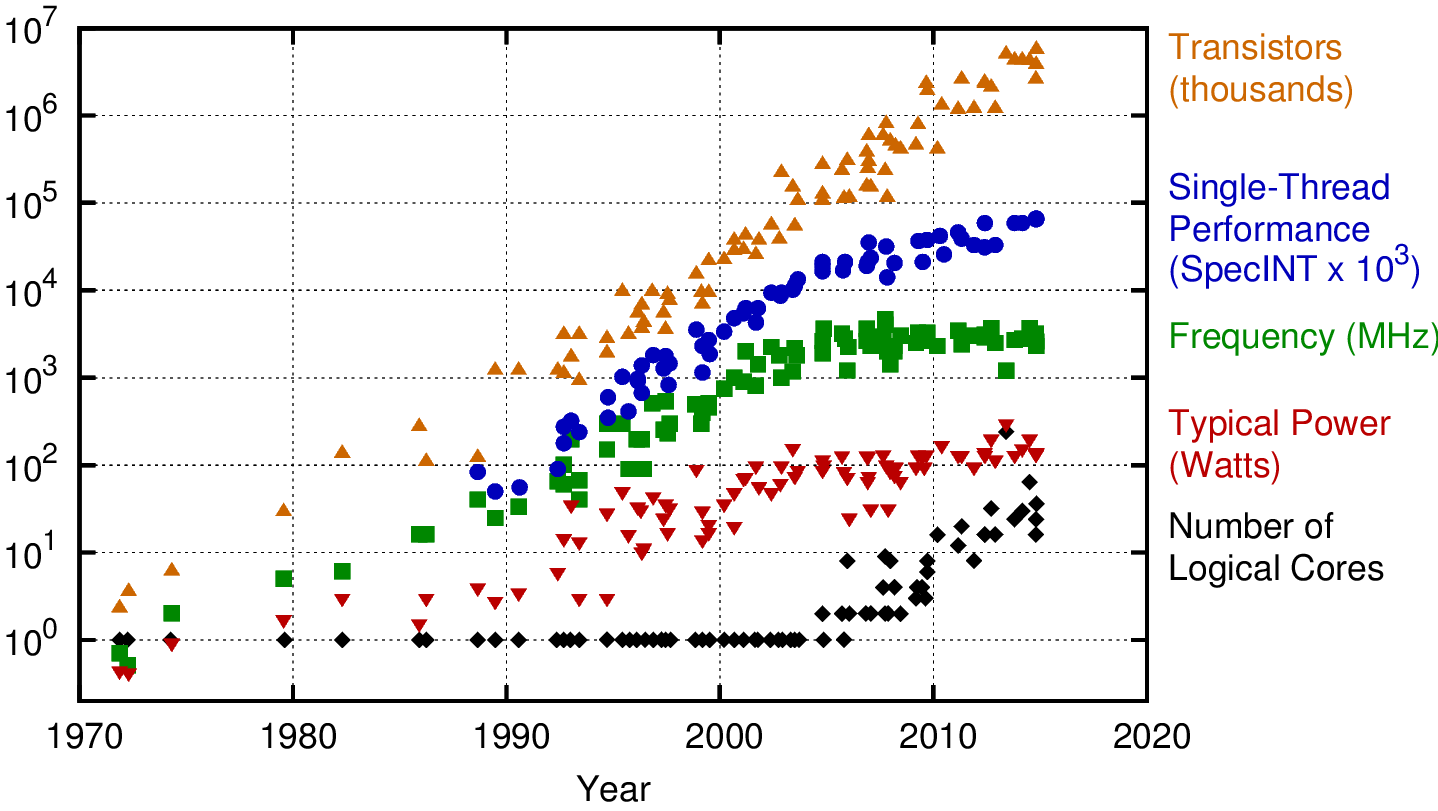
\includegraphics[width=\textwidth]{cpu_trend.png}
    \caption{
        Trend in performance of CPUs over the last 40 years. 
        Data up to the year 2010 collected by M. Holowitz, F. Labonte, O. Shacham, K. Olukotun, L. Hammond, and C. Batten. 
        Data after the year 2010 collected by K. Rupp. 
        Figure taken from \cite{Rupp}.
    } \label{fig_cpu_trend}
\end{figure}

\begin{figure}
    \centering
    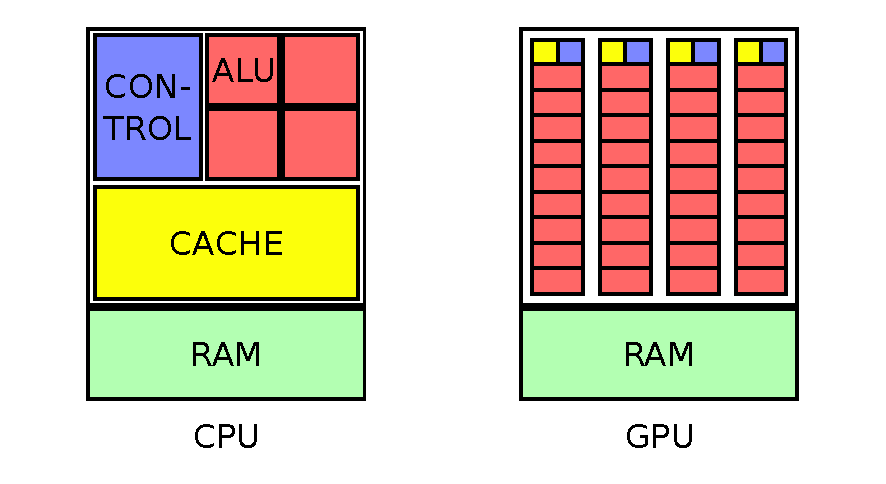
\includegraphics[]{cpu_vs_gpu.pdf}
    \caption{
        Comparison of the basic architectural differences of a CPU and a GPU.
        In green the random access memory (RAM), in yellow the cache, in blue the flow control unit and in red the arithmetic-logic unit (ALU).
        Both designs feature a RAM that all threads have access to.
        The GPU is split into many small "CPUs" (vertical groups) with their own flow control and cache.
        These are called streaming multiprocessors (SMPs or SMs).
        Generally the cache hierachry is more complicated as depicted in the figure.
        However, the defining property here is that there exists a non-global cache level that is assigned to a group of ALUs, namely the SMs. 
        Figure inspired by \cite{programming_guide}.
        } \label{fig_cpu_vs_gpu}
\end{figure}

With the invention of the MOS transistor in 1959 and more specifically the silicon-gate MOS transistor in 1968 the development of single-chip microprocessors started.
The first processors were single-threaded and clocked in the 750 kHz range (e.g. the famous Intel 4004, see \cite{Intel4004}).
However, clock rates increased exponentially over time and subsequently did the computing power (see Fig. \ref{fig_cpu_trend}).
Around 2005 this development was eventually brought to a halt in the single digit GHz regime due to physical limits of silicon. 
This is the beginning of the multi-core era. 
The idea is simple: When one thread cannot run faster, just increase the number of threads.
In 2006 the first desktop PCs with two cores were sold and ever since the number of threads is steadily increasing.
There was one problem in particular, however, that CPUs (Central Processing Unit) were not efficient in rendering graphics.
This task requires a lot of independent calculations that needed to be done in real time - a prime example for a massively parallelizable computation.
Since rendering graphics requires such a different type of computing, GPUs (Graphics Processing Unit) were developed even before the first consumer grade multi-core CPUs (e.g. the Nvidia GeForce 256 published in 1999).
These GPUs featured less single thread computation power but have a high number of threads (see Fig. \ref{fig_cpu_vs_gpu}).
State of the art GPUs have thousands of threads.
This being said, the number of threads cannot be easily compared between a CPU and a GPU or even between different GPUs as they follow different design paradigms.
How the GPU threads work will be explored in this work.
Generally, one can say that GPUs perform well in massively parallelizable computations (e.g. numerical linear algebra) while CPUs excel at single (or low number) threaded applications (e.g. running the event loop of a desktop application).
This shift to a higher number of threads rather than thread quality has been greatly motivated by scientific calculations, machine learning and computer graphics.

In this work, the basics of GPU programming in CUDA will be introduced and a very important algorithm presented, namely the tree reduction.
Using this algorithm as an example, a deeper look into the architecture of GPUs and the CUDA programming language will bring forth various optimizations.
Finally, the highly optimized implementation of the tree reduction will be tested on a consumer grade setup and a high-performance computer and the results will be discussed.

\section{Introduction to CUDA}
Unlike C code for CPUs, which will likely port to another CPU without any modification, GPU code is delicately dependent on the underlying hardware.
Different GPU developers use different application programming interfaces (APIs).
The leading GPU designer Nvidia developed a framework called CUDA, which will be used in this work.
It is simple to learn, offers efficient implementations and a plethora of literature and support.
The downside is that it only supports Nvidia GPUs and is not open source.
An alternative would be OpenCL, which is open-source but harder to learn, or HIP, which is the CUDA equivalent by AMD and very similar to it.

CUDA works as an extension to the C programming language and comes with its own compiler.
Sections of code are distributed to either the CPU (called host) or the GPU (called device).
When only writing code for the host ordinary C is used.
Writing device code is different, since the API forces the programmer into using the parallel structure of the device.
The programmer first needs to identify a section in his code that they want to parallelize - this has to be a for-loop.
This for-loop is rewritten as a so-called kernel.
They must transfer required data to the memory of the GPU and call the kernel.
When calling the kernel, the boundaries of the for-loop are set.
The loop is then executed in parallel on the GPU.
This API only allows parallelization of for-loops.
While this might seem like a very strict limitation, it closely relates to how a Nvidia GPU works.

The GPU can be thought of being organised in streaming multiprocessors (SMPs or SMs), warps and threads.
Warps will be explained in more detail later.
A SM groups a set of CUDA-cores together (of which the ALU is the central element) and allows synchronization between them.
Threads running on CUDA-cores of different SMs cannot be synchronized.
Also, threads within a SM share a cache, which cannot be accessed by threads of another SM.
The domain of the for-loop is organised in blocks and threads, where the threads are grouped in blocks.
The blocks are executed by the SMs, which means that only threads within a block can be synchronized and have access to the same cache.
This will become clearer in the next chapter.
